\documentclass{standalone}
\usepackage{tikz}
\usepackage{pgfplots}
\pgfplotsset{compat=newest}
\usepackage{amsmath}
\usepackage[american]{circuitikz}
\usepackage{cmbright}

\definecolor{myred}{RGB}{170,0,0}
\definecolor{myblue}{RGB}{0,0,220}
\definecolor{mygreen}{RGB}{0,150,0}
\definecolor{myorange}{RGB}{255,127,0}
\definecolor{mybrown}{RGB}{150,75,0}

\ctikzset{bipoles/resistor/height=0.2}
\ctikzset{bipoles/resistor/width=0.5}

\begin{document}
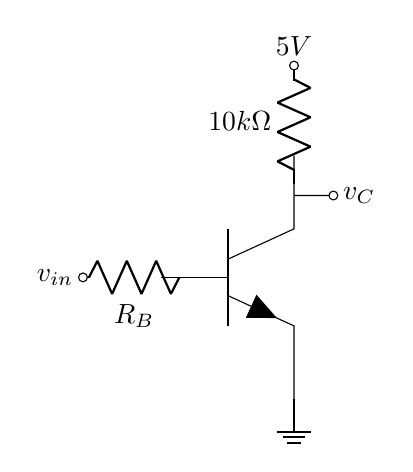
\begin{tikzpicture}
    \begin{scope}
        \draw (0, 0) node[npn, scale=2.0] (Q) {};
        \draw ($(Q.base) + (0.3, 0)$) 
            to[R, R={$R_B$}, -o] ++(-1.3, 0)
            node[anchor=east] {$v_{in}$};
        \draw ($(Q.collector) + (0, -0.35)$)
            to[R, -o, l={$10k\Omega$}] ++(0, 1.5)
            node[anchor=south] {$5V$};
        \node[ground] at (Q.emitter) {};
        \draw ($(Q.collector) + (0, -0.5)$)
            to[short, -o] ++(0.5, 0)
            node[anchor=west] {$v_{C}$};
    \end{scope}
\end{tikzpicture}
\end{document}